\section{Derivable functions}
In this section, we state the main result of this paper: the  first-order tree-to-tree transductions are exactly the class which is obtained by starting with certain prime functions (such as depth-first traversal) and applying certain  combinators (such as function composition). 

\subsection{Datatypes}
\label{sec:datatype-constructors}
 Our goal is to describe tree-to-tree functions. However, we will decompose the functions, so that the   intermediate functions will work on other datatypes, such as pairs of trees or trees of trees etc. These datatypes  can be encoded in trees, but such encoding would be cumbersome. Following~\cite{bojanczykRegularFirstOrderList2018}, we  introduce additional  datatype constructors, such as pairing.

All datatypes represent ranked sets, i.e.~each element of a datatype has an arity. The atomic datatypes are finite ranked sets, e.g.~alphabets for trees. 

\paragraph*{Terms.} The most important datatype constructor is the  \emph{term} constructor. Terms generalise trees, by allowing for dangling edges, called ports. We allow ports so that we can decompose trees (and even terms) into smaller pieces, as  illustrated by the figure below. 
% Each  part of the tree is not a tree as it has dangling ports.  We call \emph{terms} such trees with ports. 
\begin{center}
\includegraphics[scale=.32, page=15]{pics.pdf}
\end{center}
Formally speaking, terms are defined by induction: a term over a (possibly infinite) ranked set $\rSigma$ is either a term which consists only of a port, 
or it is an expression of the  form $a \tensorpair{t_1,\ldots,t_n}$ where $a \in \rSigma$ has arity $n$, and $t_1,\ldots,t_n$ are already defined terms. The arity of a term is the number of ports. Terms of arity zero are the same as trees. We write $\tmonad \rSigma$ for the ranked set of terms over an ranked set $\rSigma$.    Terms form a monad, in the category of ranked sets and arity-preserving functions. The unit of the monad, which is an operation of type $\ranked{\rSigma \to \tmonad \rSigma}$, is illustrated in the following picture:
\mypic{98}
The product of the monad, which is an operation of type $\ranked{\tmonad \tmonad \rSigma \to \tmonad \rSigma}$ that we call \emph{flattening}, is illustrated in the following picture:
\mypic{97}

\paragraph*{Products and coproducts.}
We have two binary datatype constructors
\begin{align*}
\underbrace{\ranked{\Sigma_1 \otimes \Sigma_2}}_{\text{tensor product}} \qquad \underbrace{\ranked{\Sigma_1 + \Sigma_2}}_{\text{coproduct}}
\end{align*}
An element of the tensor product is a pair $\tensorpair{a_1,a_2}$ where $a_i \in \ranked{\Sigma_i}$. The arity of the pair is the sum of arities of $a_1$ and $a_2$. We draw pairs like this:
\mypic{52}     
An element of the coproduct is a pair $(i,a)$ where $i \in \set{1,2}$ and $a \in \ranked{\Sigma_i}$. The arity is inherited from $a$. 

The set of terms can be phrased in terms of tensor products and coproducts, as the least solution of the equation:
\begin{align*}
\tmonad \rSigma = \overbrace{\redset{\portletter}}^\text{port}  \ranked{+\coprod_{\black {a \in} \rSigma}} \overbrace{\ranked{\tmonad \rSigma \otimes \cdots \otimes \tmonad \rSigma}}^{\text{arity of $a$ times}}
\end{align*}  where $\ranked \coprod$ denotes possibly infinite coproduct.

\paragraph*{Folding.}
The final datatype constructor called \emph{folding}. Folding has two main purposes: (1) reordering ports in a term; and (2) reducing arities by grouping ports into groups. More formally, there is one unary constructor $\reduce k \rSigma$ for every $k \in \set{1,2,3,\ldots}$.  An $n$-ary element of $\reduce k \rSigma$, which is called a \emph{$k$-fold}, consists of an element      $a \in \rSigma$  together with an  injective \emph{grouping}  function
\begin{align*}
    f : \set{1,\ldots,\arity a} \to \underbrace{\set{1,\ldots,n}}_{\text{which group}} \times  \underbrace{\set{1,\ldots,k}}_{\substack{\text{which position}\\ \text{in the group}}}.
\end{align*}
We denote such an element as $a/f$ and draw it like this: \mypic{53}
In the above picture there are $n=4$ groups of $k=3$ elements. The arity of $a$ is 5, and the 5 ports of $a$ are mapped by the grouping function to pairs (group, position) according to the lines in the picture. 

Already for $k=1$, the constructor $\reduce 1$ is non-trivial, since it can reorder ports (using a non-monotone grouping function), or add dummy ports (using a non-surjective grouping function).
When viewed as a family of datatype constructors,  folds have a monad-like structure -- they are a graded  monad~\cite[p. 518]{fujiShinyaMellies2016}. The unit is the operation 
\mypic{98}
of type $\ranked{\Sigma \to \reduce 1 \Sigma}$, while  the product (or flattening) is the family of operations $\ranked{\reduce k \reduce m \Sigma \to \reduce {k \cdot l} \Sigma}$, indexed by $k,l \in \set{1,2,\ldots}$ that is illustrated in the following picture:
\mypic{99}
More formally, the flattening of two folds $(a/f)/g$ has the grouping function defined by
\begin{align*}
i \mapsto (x', \!\!\!\!\overbrace{(y',y)}^{\substack{\text{represented}\\ \text{as a number in}\\ \text{$\set{1,\ldots,kl}$}}}\!\!\!\!) \qquad \text{where} \begin{cases}
    (x,y) &= f(i)\\
    (x',y') &= g(x)
\end{cases}
\end{align*}
% $k=2$, $n=4$, and $a$ has arity $a$. There  The groups are  and the arity of $a$ is 6, and $f$ is
% \begin{align*}
% \begin{array}{rccccccc}
%     i \in \set{1,\ldots,\arity a} &  \quad &1 & 2 & 3 & 4 & 5 & 6\\
%     \text{group of $f(i)$} &  & 1 & 1 & 4 & 2 & 3 & 4\\
%     \text{position of $f(i)$} & & 2 & 1 & 1 & 2 & 1 & 2 
% \end{array}
% \end{align*}
% A term has an arity, which is  the number of ports. Because the set of terms is itself a ranked set,  we can create terms of terms.  In fact, all of the datatypes and datatype constructors  work with ranked sets.


% A consequence of using terms is that we  work in the category of ranked sets; i.e.~our datatypes represent ranked sets and the functions we consider are arity-preserving functions between ranked sets.  As mentioned before, we use  red for ranked sets; we also use red  for operations that output ranked sets. 

%\footnote{This is a difference of trees as opposed to strings~\cite{bojanczykRegularFirstOrderList2018}, where ranked sets are not needed, because a part of a string is also a string.}
 
%
%
%The crucial property of the prime functions and  the combinators is that they use ranked sets. This is because the type constructor of this paper, namely terms, uses ranked sets.  Roughly speaking, a term is a tree with missing parts. The missing parts arise when we  isolate smaller parts of a bigger tree, as illustrated in the following picture:




%\begin{definition}[Terms]\label{def:terms}
%    An  term\footnote{
%        Our definition of terms differs from the definition used in universal algebra. An $n$-ary term in the sense of this paper is, in the language of universal algebra, a term over variables $\set{x_1,\ldots,x_n}$ where each variable appears exactly once, and the variables are used from left to right.  The requirement that variables appear  once is related to the linear output size of first-order tree-to-tree transductions. Without this requirement, even homomorphisms would have exponential output size. 
%    } over a ranked set $\rSigma$ is a tree over alphabet $\rSigma \redplus \redzero$, where $\redzero$ is a set with one element of arity zero.  The nodes with labels from $\redzero$  -- which are leaves --  are called \emph{ports}. The arity of a term is the number of ports.  We write $\tmonad \rSigma$ for the ranked set of terms over $\rSigma$.  
%\end{definition}




\paragraph*{Datatypes.} This completes the list of  datatype constructors. The datatypes are then defined by applying the constructors to the prime datatypes, which are either finite ranked sets (those with finitely many elements), or  the terminal ranked set (i.e.~a ranked set which admits a unique function from every other ranked set).
% We call such ranked sets \emph{types}.
%  The general idea is that we start with finite ranked sets, and close these under the following type constructors: coproducts, two kinds of product (Cartesian and tensor), taking terms, and a type constructor that allows to merge ports.
%  and the matrix power. 
% The  matrix power -- which is possibly the least natural type constructor -- will be motivated and discussed in more detail later on.



\begin{definition}[Datatypes] \label{def:types} A \emph{datatype} is any ranked set which can be obtained by applying the constructors 
    \begin{align*}
    \ranked{\tmonad \rSigma \qquad \rSigma_1 \otimes \rSigma_2 \qquad \rSigma_1 + \rSigma_2 \qquad \reduce k \rSigma},
    \end{align*}
    to ranked sets which are either finite or equal to 
    \begin{align*}
    \termset \eqdef  \underbrace{\redset{\naryterm 0, \naryterm 1, \naryterm 2,\ldots}.}_{\substack{\text{for each arity $i$, one} \\ \text{element denoted by $i$}}}
    \end{align*}
\end{definition}

\subsection{Derivable functions}
\smallskip
\newcommand{\funcitem}[3]{\ranked{#1  } &:& \ranked{#2} \rto  \ranked{#3}}
This completes the definition of the datatype constructors. 
All datatype constructors are functors, in the sense  that  arity preserving functions
\begin{align*}
\ranked{f_1 : \Sigma_1 \to \Gamma_1 \qquad f_2 : \Sigma_2 \to \Gamma_2}
\end{align*}       
can be lifted, in the natural way, along the type constructors to new arity preserving  functions
\begin{eqnarray}
\label{eq:liftplus}\funcitem{f_1 + f_2}{\Sigma_1 + \Sigma_2}{\Gamma_1 + \Gamma_2} \\
\funcitem{\tensorpair{f_1,f_2}}{\Sigma_1 \otimes \Sigma_2}{\Gamma_1 \otimes \Gamma_2}\\
\funcitem{\reduce k f_1}{\reduce k \Sigma_1}{\reduce k \Gamma_1}\\
\funcitem{\tmonad f_1}{\tmonad \Sigma_1}{\tmonad \Gamma_1}
%\\\label{eq:liftshallow}\funcitem{\shallowterm{f_1}{f_2}}{\shallowterm{\Sigma_1}{\Sigma_2}}{\shallowterm {\Gamma_1}{\Gamma_2}} 
\end{eqnarray}

We now introduce the main new definition of this paper.

\begin{definition}[Derivable function]
    The class of \emph{derivable} functions is the least class which contains:
    \begin{itemize}
    \item for every $\rSigma$, the unique arity preserving function $\ranked{\Sigma \to \termset}$;
    \item  all arity preserving functions with finite domain;
        \item  the prime functions in Figures~\ref{fig:monad},\ref{fig:product} and \ref{fig:not-explained};
         \end{itemize}
and which is closed under composition and  liftings (1)--(4).
\end{definition}

%
\newcommand{\fotitem}[2]{$\displaystyle #1$ & #2 \\ \\ }
\begin{figure}[h]
    \centering 
    \begin{tabular}{ll}
        \fotitem{
            \frac
            { \ranked{f : \Sigma \to \Delta} \quad \ranked{g : \Delta \to \Gamma}}
            {\ranked{g \circ f :  \Sigma \to  \Gamma}}
            }
            {
                Composition of functions.
            }
        \fotitem{
            \ranked{f : \Sigma \to \Gamma}
            }
            {
                Every arity preserving function with finite domain $\rSigma$.
            }
            \fotitem{
                \ranked{\iota_i : \Sigma_i \to \Sigma_1 + \Sigma_2}
                }
                {
                    Coprojection for $i \in \set{1,2}$.
                }
        \fotitem{
            \frac
            { \ranked{f_1 : \Sigma_1 \to \Gamma} \quad \ranked{f_2 : \Sigma_2 \to \Gamma}}
            {\ranked{f_1 \text{or} f_2 :  (\Sigma_1 + \Sigma_2) \to  \Gamma}}
            }
            {
                Co-pairing of functions.
            }
            \fotitem{
                \ranked{\pi_i : \Sigma_1 \times \Sigma_2 \to \Sigma_i}
                }
                {
                    Projection for $i \in \set{1,2}$.
                }
        \fotitem{
            \frac
            { \ranked{f_1 : \Sigma \to \Gamma_1} \quad \ranked{f_2 : \Sigma \to \Gamma_2}}
            {\ranked{(f_1,f_2) :  \Sigma \to  \Gamma_1 \times \Gamma_2}}
            }
            {
                Pairing of functions.
            }
            \fotitem{
                \ranked{\distrcart : (\Sigma_1 + \Sigma_2)\times \Gamma \to (\Sigma_1 \times \Gamma) + (\Sigma_2 \times \Gamma)}
                }
                {
                    Cartesian product distributes across coproduct.
                }
            \fotitem{
            \frac
            { \ranked{f_1 : \Sigma_1 \to \Gamma_1} \quad \ranked{f_2 : \Sigma_2 \to \Gamma_2}}
            {\ranked{ \tensorpair{f_1,f_2}  :  \Sigma_1 \otimes \Sigma_2 \to  \Gamma_1 \otimes \Gamma_2}}
            }
            {
                Lifting functions to tensors.
            }
            \fotitem{
                \ranked{\distrtensor : (\Sigma_1 + \Sigma_2)\otimes \Gamma \to (\Sigma_1 \otimes \Gamma) + (\Sigma_2 \otimes \Gamma)}
                }
                {
                    Tensor product distributes across coproduct.
                }
            \fotitem{
            \frac{ \ranked{f : \Sigma \to \Gamma}}{\ranked{\tmonad f : \tmonad \Sigma \to \tmonad \Gamma}}
            }
            {
                Lift a function from the alphabet  to terms.
            }
            \fotitem{
            \ranked{\unit_\Sigma : \Sigma \to \tmonad \Sigma}
            }
            {
                View a letter as a term.
            }
            \fotitem{
                \ranked{\flatt_\Sigma : \tmonad \tmonad \Sigma \to \tmonad \Sigma}
                }
                {
                    Flatten a term of terms into a term.
                }
                \fotitem{
                \ranked{ \composeterm :  
                \set * + \coprod_{a \in \Sigma} \overbrace{\tmonad \rSigma \otimes \cdots \otimes \tmonad \rSigma}^{\text{arity of $a$ times}} \to \tmonad \rSigma }
                }
                {
                        Compose a term from its list of children, for finite $\rSigma$.
                }
            \fotitem{
                \ranked{ \decomposeterm : \tmonad \rSigma \to 
                \set * + \coprod_{a \in \Sigma} \overbrace{\tmonad \rSigma \otimes \cdots \otimes \tmonad \rSigma}^{\text{arity of $a$ times}}}
                }
                {
                        The inverse of $\composeterm$, for finite $\rSigma$.
                }    
    
            \fotitem{
                \ancfact, \decfact  : \ranked{\tmonad(\Sigma_1+\Sigma_2) \to \tmonad(\tmonad \Sigma_1 + \tmonad \Sigma_2)}
            }
                    {
                        Ancestor and descendant factorisations.
                    }
            \fotitem{
                \ranked{\preorder : \tmonad \Sigma \to \tmonad (\rSigma + \set{\grayball, \grayballbin})}
                }
                {
                    Pre-order traversal.
                }    
            % \fotitem{
            %     \ranked{\unfold : \tmonad (\Sigma^{[k]}) \to (\tmonad \Sigma)^{[k]}}
            % }
            %     {
            %             Matrix power distributes across terms.
            %     }
    \end{tabular} 
    
    \caption{First-order term functions}
    \label{fig:fo-term}
\end{figure}

The prime functions in Figure~\ref{fig:monad} describe the monad structure of terms and folds, and were explained in Section~\ref{sec:datatype-constructors}. The prime functions in Figure~\ref{fig:product} are  simple syntactic transformations, which are intended to have no computational content.  Figure~\ref{fig:not-explained} contains   less obvious operations, whose definitions are  deferred to Section~\ref{sec:prime-and-combinators}. Before giving these definitions, we state the main result of the paper. 

% \begin{example}
%     To get a feeling for the prime functions and combinators, we derive the function
%     \begin{align*}
%     \tensorpair{a,b} \in \ranked{\rSigma^2} \qquad \mapsto \qquad  \tensorpair{b,a} \in \ranked{\rSigma^2}
%     \end{align*}
%     which witnesses commutativity of the product for pairs of the same type. The idea is to embed pairs into terms, and use simple manipulations on terms. 
%     We  draw the unique elements of the sets $\redzero$, $\redone$ and $\redtwo$ as follows:
%     \mypic{79}
%     We begin by deriving a function which maps a tensor pair into a shallow term whose root is the unique element of $\redtwo$.  This is achieved by composing the derivable functions of types 
%     \begin{align*}
%     \ranked{
%         \xymatrix{
%             \rSigma \otimes \rSigma \ar[r] &
%             (\shallowterm \redone \rSigma) \otimes (\shallowterm \redone \rSigma) \ar[r] &
%             \shallowterm{(\redone \otimes \redone)}  {(\rSigma+\rSigma)} \ar[r] & \shallowterm \redtwo \rSigma
%         }
%     }
%     \end{align*}
%     which is described in the following picture:
%     \mypic{78}
%     The last function applies the bijection $\ranked{\redone \otimes \redone \to \redtwo}$, which is derivable by virtue of having a finite domain. 

%     Next, we can swap the children of 
% \end{example}

% We first observe that terms and unary folding are monads. 
% The monad structure for terms is induced by:
% \begin{align*}
%         \underbrace{\ranked {\tmonad f : \tmonad \Sigma \to \tmonad \Gamma}}_{\text{$\tmonad$ is a functor}} \qquad  \underbrace{\unit_\rSigma : \rSigma \rto \tmonad \rSigma}_{\text{the unit in the monad}} \qquad  \underbrace{\flatt_\rSigma : \tmonad \tmonad \rSigma \rto \tmonad \rSigma}_{\text{the product operation in the monad}},
% \end{align*}
% and a similar situation holds for unary folds $\reduce 1$.  More generally, the family of folds $\set{\reduce k}_{k}$ is a graded monad. Finally, the operation $\tmonad \reduce 1 \rSigma \rto \reduce 1 \tmonad \rSigma$ is a distributive law of these two monads.

% For a derivable function, its domain and co-domain are types as in Definition~\ref{def:types}, in particular the domain and co-domain are ranked sets. The prime functions are arity-preserving and the combinators preserve this property, and therefore all derivable functions are arity-preserving. 


% We are now ready to state the main theorem of this paper. 

\begin{theorem}\label{thm:main}
    Let $\rSigma,\rGamma$ be finite ranked sets. A function 
    \begin{align*}
        f : \trees \rSigma \to \trees \rGamma
    \end{align*}
    is a first-order tree-to-tree transduction if and only if it is the restriction to trees of some derivable
    \begin{align*}
        \ranked {f : \tmonad \Sigma \to \tmonad \Gamma}.
    \end{align*}
    
\end{theorem}

The bottom-up implication in the above theorem is proved by a straightforward induction on the derivation. We associate to each datatype a relational structure; for example the relational structure associated to a pair $\tensorpair {a_1,a_2}$ is the disjoint union of the relational structures associated to $a_1$ and $a_2$. These relational structures can then be transformed using first-order transductions.   We then show that all prime functions are first-order transductions (adapted suitably to structures other than trees); and that this property is preserved under applying the combinators.  This proof is in the appendix, and the rest of the paper is devoted to the top-down implication in the theorem, which says that every first-order transduction can be decomposed into the prime functions.
%\subsection{Proposition of another presentation of prime functions}
\begin{figure}
\fbox{
\begin{minipage}{1\linewidth}
\begin{itemize}
\item \textbf{Unit and product in  the monad $\tmonad$.} 
        $$\begin{array}{rlllcrlll}
\unit: &\rSigma &\ranked{\to} & \tmonad \rSigma & \qquad &
\flatt: &\tmonad\tmonad\rSigma &\ranked{\to} & \tmonad \rSigma
% \\[2pt]
% &a &\mapsto& a\tensorpair{\portletter,\dots,\portletter}
       \end{array}$$ 
\item \textbf{Unit and product in the graded monad $\reduce k$.} 
        $$\begin{array}{rlllcrlll}
\unit: &\rSigma &\ranked{\to} & \reduce 1 \rSigma & \qquad &
\flatt: &\reduce k \reduce l \rSigma &\ranked{\to} & \reduce {k.l} \rSigma 
% \\[2pt]
% &a &\mapsto& a/(i\mapsto(i,1))
       \end{array}$$ 
       \item \textbf{Inductive structure of terms (for finite $\rSigma$ only).}
       $$\begin{array}{cc}
        \ranked{
        \xymatrix@C=2cm{
\tmonad \Sigma \ar@<.5ex>[r]^-{\text{decompose}}
        & 
        \ar@<.5ex>[l]^-{\text{compose}}
        \redset{\portletter}  +\coprod_{\black {a \in} \rSigma}} 
        \powersmall{(\tmonad \rSigma)}{\text{arity of $a$}}
        } 
    \end{array}$$ 
    \item \textbf{Remove unused fold.}
    $$\begin{array}{rlll}
         &\reduce k \rSigma &\ranked{\to} &  \ranked{\rSigma + \termset}
         \\[2pt]
         &(a/f) &\mapsto& \text{$a$ if $a$ has arity 0, undefined otherwise}
               \end{array}$$ 
\end{itemize}
\end{minipage}
}
\caption{Prime functions for terms and fold.}\label{fig:monad}
\end{figure}

% \miktodo{Seems that were are missing projections and co-projections for $\product$}
\begin{figure}
\fbox{
\begin{minipage}{1\linewidth}
\begin{itemize}
\item \textbf{Co-projections.} 
$$
\begin{array}{llllll}
\ranked{\rSigma + \rSigma} &\ranked{\to} & \rSigma \qquad & \qquad \ranked{\rSigma_i}  &\ranked{\overset{\iota_i}{\to}} & \ranked{\rSigma_1 + \rSigma_2} \\[0pt]
(a,i)&\mapsto& a   \qquad & \qquad  a &\mapsto& (a,i) 
       \end{array}
$$
\item \textbf{Commutativity.} 
$$
\begin{array}{rllrll}
\ranked{\rSigma + \rGamma} &\ranked{\to} & \ranked{\rGamma + \rSigma} \qquad & \qquad \ranked{\rSigma \product \rGamma} &\ranked{\to} & \ranked{\rGamma \product \rSigma} \\[0pt]
(a,1)&\mapsto& (a,2)  \qquad & \qquad
\tensorpair{a,b}&\mapsto& \tensorpair{b,a}\\
(a,2)& \mapsto& (a,1)
       \end{array}
$$
\item \textbf{Associativity.}
$$
\begin{array}{rllrll}
\ranked{(\rSigma + \rGamma) + \rDelta} &\hspace{-.2cm}\ranked{\to}&\hspace{-.2cm} \ranked{\rGamma + (\rSigma+\rDelta)}  & \ranked{(\rSigma \product \rGamma) \product \rDelta} &\hspace{-.2cm}\ranked{\to}&\hspace{-.2cm} \ranked{\rSigma \product (\rGamma \product \rDelta)} \\[2pt]
 ((a,1),1)&\hspace{-.2cm}\mapsto&\hspace{-.2cm} (a,1) & 
\tensorpair{\tensorpair{a,b},c}&\hspace{-.2cm}\mapsto&\hspace{-.2cm}\tensorpair{a,\tensorpair{b,c}}\\[2pt]
         ((a,2),1)&\hspace{-.2cm}\mapsto&\hspace{-.2cm}((a,1),2) & & &\\[2pt]
         (a,2) &\hspace{-.2cm}\mapsto&\hspace{-.2cm} ((a,2),2) & & &
       \end{array}
$$
\item \textbf{Distributivity.}
$$\begin{array}{rll}
\ranked{(\Sigma_1 + \Sigma_2)\product \Gamma }& \ranked{\to} &\ranked{(\Sigma_1 \product \Gamma) + (\Sigma_2 \product \Gamma)}\\[2pt]
\tensorpair{(a,i),b}&\mapsto& (\tensorpair{a,b},i)
\end{array}$$
\end{itemize}
\end{minipage}
}
\caption{Prime functions for product and coproduct.}\label{fig:product}
\end{figure}

\begin{figure}
\fbox{
\begin{minipage}{1\linewidth}
\begin{itemize}
\item \textbf{Factorisations.}
$$\begin{array}{cc}
        \ranked{
        \xymatrix@C=1cm{
\tmonad(\Sigma_1+\Sigma_2) \ar@<.5ex>[r]^{ \ancfact}
        \ar@<-.5ex>[r]_{\decfact}& \tmonad(\tmonad \Sigma_1 + \tmonad \Sigma_2)
        }}
    \end{array}$$ 
\item \textbf{Pre-order.} (Here $\grayball, \grayballbin$ are letters of arities $0,2$).
$$\begin{array}{cc}
        \ranked{
        \xymatrix@C=.7cm{
\tmonad \Sigma \ar[r]& \reduce 1 \tmonad(\rSigma + \redset{\grayball,\grayballbin})
        }} 
    \end{array}$$ 
\item \textbf{Monotone unfolding.}
$$\begin{array}{cc}
        \ranked{
        \xymatrix@C=.7cm{
 \tmonad \reduce k \powersmall \Sigma k \ar[r]& \reduce k \powersmall{(\tmonad \rSigma)} k  +  \termset 
        }}
    \end{array}$$ 
\end{itemize}
\end{minipage}
}
\caption{Functions explained in Section~\ref{sec:prime-and-combinators}. }\label{fig:not-explained}
\end{figure}



%\begin{figure}
\fbox{
\begin{minipage}{1\linewidth}
\begin{itemize}
\item \textbf{Unit.}
$$
\begin{array}{c}
 \ranked{\Sigma} \ \ \ranked{\leftrightarrow} \ \    \ranked{ \Sigma \cdot 1}\\[5pt]
        {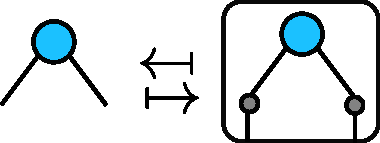
\includegraphics[scale=.4]{pictures/sigma-dot-1}} 
\end{array}
$$
\item \textbf{Associativity.}
$$
\begin{array}{c}
 \ranked{(\Sigma \cdot \Gamma)\cdot \Delta } \ \ \ranked{\to} \ \    \ranked{ \Sigma \cdot (\Gamma \cdot \Delta)}\\[5pt]
        {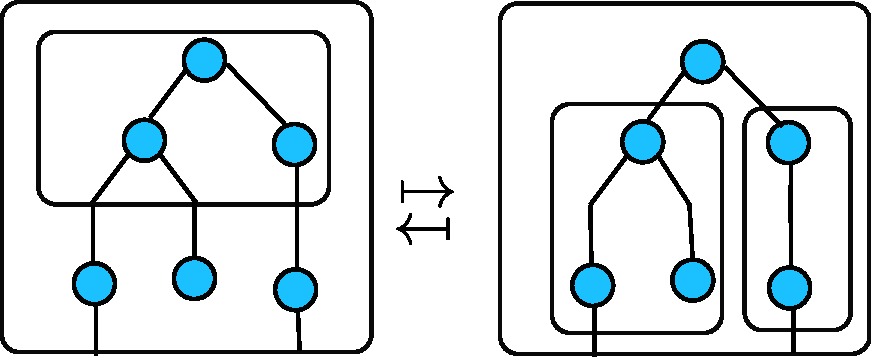
\includegraphics[scale=.4]{pictures/associativity-shallow}} 
\end{array}
$$
\item \textbf{Terms as shallow terms.}
$$
\begin{array}{c}
 \ranked {1 + \shallowterm \Sigma {\tmonad \Sigma}\ \ \to \ \  \tmonad \Sigma}\\[5pt]
        {
        \begin{tabular}{l}
            Every term is either just a port,\\ or has a root and child subterms.    
        \end{tabular}    
        }
\end{array}
$$
\item \textbf{Tensors as shallow terms.}
$$
\begin{array}{c}
\ranked {\Sigma^n \ \ \leftrightarrow \ \ \shallowterm n \Sigma}\\[5pt]
        {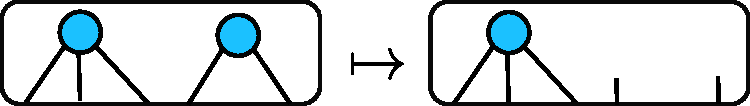
\includegraphics[scale=.4]{pictures/tensor-projection-1}}
\end{array}
$$
\end{itemize}
\end{minipage}
}
\caption{Prime functions for shallow terms.}\label{fig:prime-for-shallow-terms}
\end{figure}

\begin{figure}
\fbox{
\begin{minipage}{1\linewidth}
\begin{itemize}
\item \textbf{Unit.}
$$
\begin{array}{c}
 \ranked{\Sigma \ \ \to \ \ \reduce k \Sigma^k}\\[5pt]
        {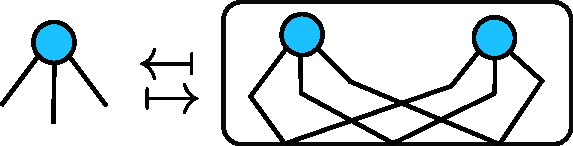
\includegraphics[scale=.4]{pictures/tensor-injection}}
\end{array}
$$
\item \textbf{Increase fold.}
$$
\begin{array}{c}
 \ranked{\reduce k \Sigma \ \ \to \ \ \reduce {k+1}\Sigma}\\[5pt]
        {
\includegraphics[scale=.4]{pictures/add-fold}}	
\end{array}$$
\item \textbf{Decrease fold.}
$$
\begin{array}{c}
 \ranked{\reduce {k+1} \Sigma \ \ \to \ \ \reduce {k}\Sigma+\bot}\\[5pt]
        {
\includegraphics[scale=.4]{pictures/reduce-fold}}	 
\end{array}$$
\item \textbf{projection of copairs.}
$$
\begin{array}{c}
   \ranked{\Sigma\product \Sigma \ \ \to \ \ \reduce 1 \Sigma}\\[5pt]
        {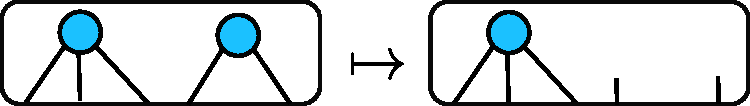
\includegraphics[scale=.4]{pictures/tensor-projection-1}}	
\end{array}$$
\end{itemize}
\end{minipage}
}
\caption{Additional prime functions for folds.}\label{fig:additional-prime-for-fold}
\end{figure}

\begin{figure}
\fbox{
\begin{minipage}{1\linewidth}
\begin{itemize}
\item \textbf{Folds over pairs.}
$$
\begin{array}{rll}
  \ranked{\reduce k (\Sigma_1 + \Sigma_2)}& \ranked{\to} & \ranked{\reduce k \Sigma_1 + \reduce k \Sigma_2}\\
         (a,i)/f & \mapsto & ((a/f),i)
\end{array}
$$
\item \textbf{Shallow terms over pairs.}
$$
\begin{array}{rll}
  {\shallowterm {(\Sigma_1 + \Sigma_2)} \Gamma} & \ranked{\to} & \ranked{(\shallowterm {\Sigma_1} \Gamma) + (\shallowterm {\Sigma_2} \Gamma)}\\
        (a,i)\tensorpair{t_1,\dots,t_n} &\mapsto& (a\tensorpair{t_1,\dots,t_n},i)
\end{array}
$$
\item \textbf{Shallow terms over copairs.}
$$
\begin{array}{c}
  \ranked{{\shallowterm {(\Sigma_1 \product \Sigma_2)} \Gamma}
   \ \  \to \ \ {(\shallowterm {\Sigma_1} \Gamma) \product (\shallowterm {\Sigma_2} \Gamma)}}\\[5pt]
        {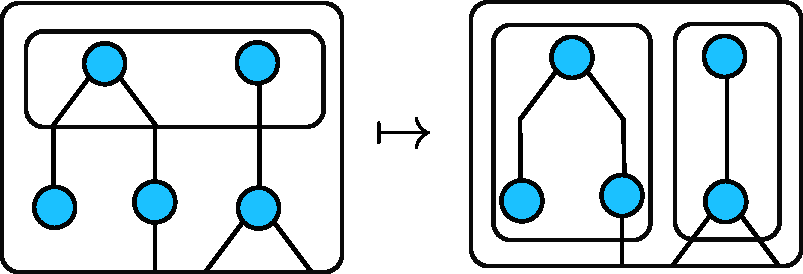
\includegraphics[scale=.4]{pictures/tensor-shallow-distrib}}
        \end{array}
$$
\item \textbf{Folds over copairs.}
$$
\begin{array}{c}
\ranked{(\reduce k \Sigma_1) \product (\reduce k {\Sigma_2}) \ \ \to \ \reduce k (\Sigma_1 \product \Sigma_2)}\\[5pt]
        {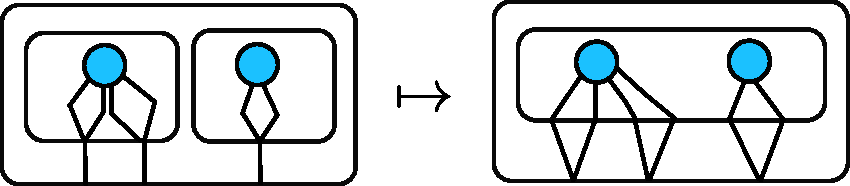
\includegraphics[scale=.4]{pictures/tensor-fold-distrib-2}}  
\end{array}
$$
\item \textbf{Folds over copairs (bis).}
$$
\begin{array}{c}
    \ranked{\reduce k (\Sigma_1 \product \Sigma_2) \ \ \to \ \ \reduce k ((\reduce k {\Sigma_1})\product (\reduce k \Sigma_2))}\\[5pt]
        {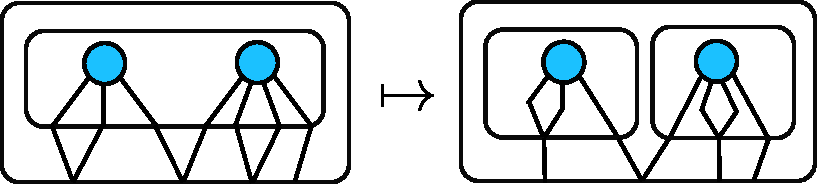
\includegraphics[scale=.4]{pictures/tensor-fold-distrib-1}}   
\end{array}
$$
\item \textbf{Shallow terms over folds.}
$$
\begin{array}{c}
 \ranked{\shallowterm \Sigma {\reduce k \Gamma}\ \ \to \ \ \reduce k (\shallowterm \Sigma {\Gamma})}\\[5pt]
 {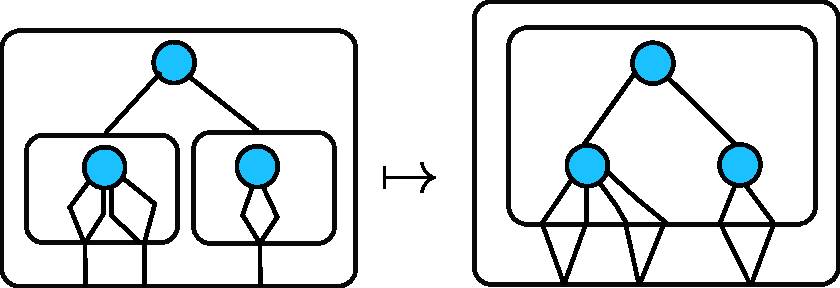
\includegraphics[scale=.4]{pictures/shallow-fold-distrib}} 
\end{array}
$$
\item \textbf{Folds over shallow terms.} 
$$
\begin{array}{c}
 \ranked{\reduce k \Sigma\cdot \Gamma\ \ \to \ \ (\reduce k \Sigma) \cdot \mati k \Gamma}\\[5pt]
 {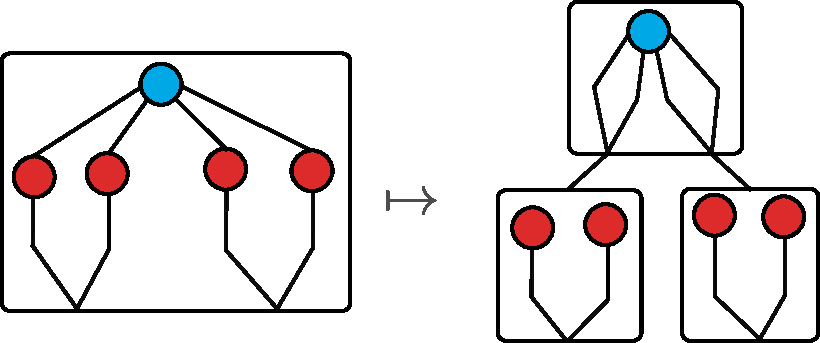
\includegraphics[scale=.4]{pictures/last-prime-function}} 
\end{array}
$$
$\rGamma$ is a set of unary elements.
\end{itemize}
\end{minipage}
}
\caption{Additional distributivity prime functions.} \label{fig:additional-distrib-prime}
\end{figure}

\begin{figure}
\fbox{
\begin{minipage}{1\linewidth}
\begin{itemize}
\item \textbf{Untwist.}
$$
\begin{array}{c}
\ranked{\tmonad {\reduce 1\Sigma} \ \  \to \ \ \reduce 1 \tmonad \Sigma}\\[5pt]
         {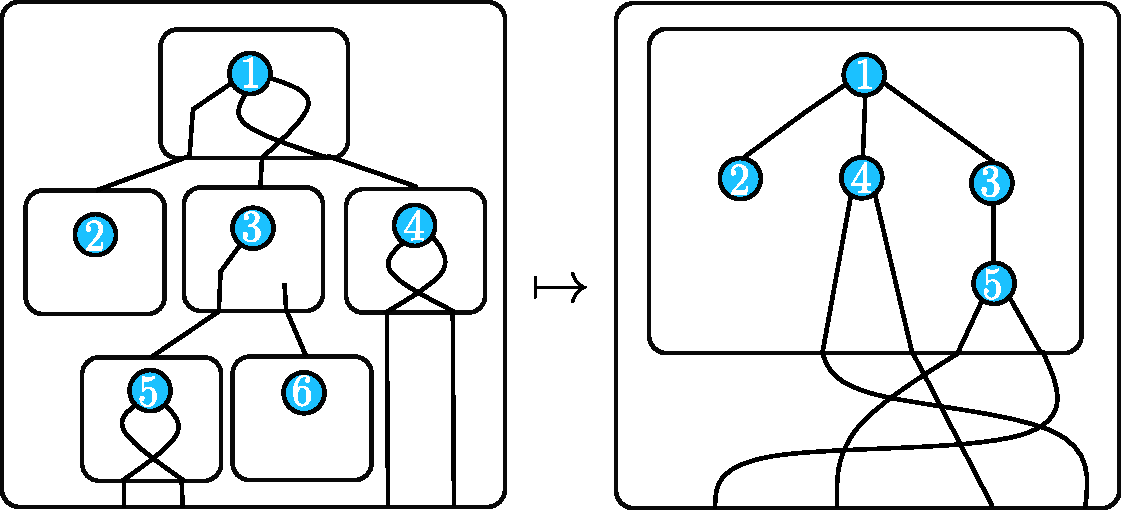
\includegraphics[scale=.4]{pictures/unfold-1}}
\end{array}
$$
\item \textbf{External fold.}
$$
\begin{array}{c}
\ranked{\tmonad {\reduce k\Sigma} \ \  \to \ \ \reduce k \tmonad \reduce k\Sigma}\\[5pt]
         {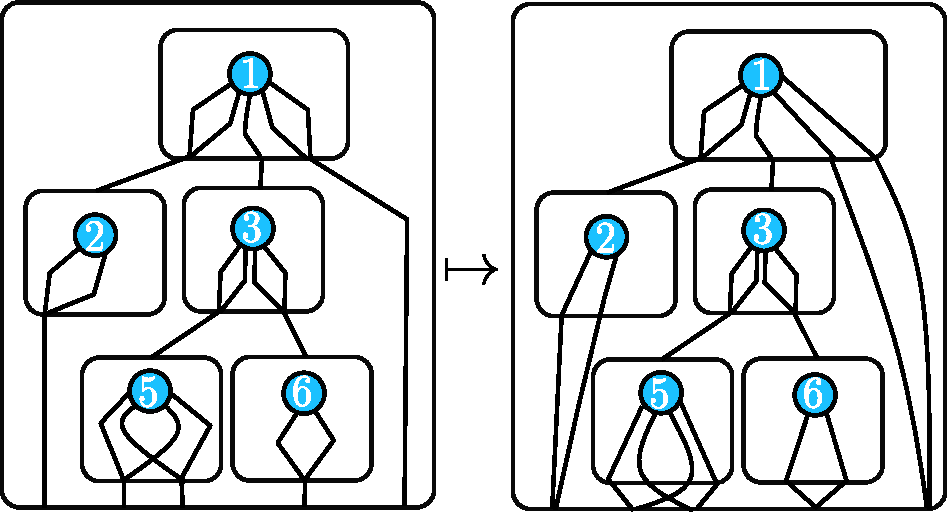
\includegraphics[scale=.43]{pictures/external-unfold-1}}
\end{array}
$$
\item \textbf{Matching.}
$$
\begin{array}{c}
\ranked{\shallowterm {\reduce k \Sigma}{\Gamma^k} \ \ \to \ \ \reduce 1(\shallowterm \Sigma \Gamma)}\\[5pt]
\includegraphics[scale=.3]{pictures/shallow-unfold}
\end{array}
$$
\end{itemize}
\end{minipage}
}
\caption{Weak forms of unfolding.}\label{fig:weak-unfolding}
\end{figure}
\subsection{The prime functions from Figure~\ref{fig:not-explained}}
\label{sec:prime-and-combinators}
Before continuing with the proof of top-down implication in Theorem~\ref{thm:main}, we  describe the prime functions from Figure~\ref{fig:not-explained}. 
Each of these functions will play a key role in one of the main results of the paper.
%  We will highlight the moments when such functions are used.  


\subsubsection{Factorisations}
    Let $t \in \tmonad \rSigma$ be a term. A factorisation of $t$ is a partition of the term into smaller terms. This can be formalised using two  equivalent definitions. One definition is that a factorisation is an equivalence relation on non-port nodes where every equivalence class is a factor (connected via the parent-child relation). The other definition is that a factorisation is any term $s  \in \tmonad \tmonad \rSigma$ which flattens to $t$. 
    The two definitions are easily seen to be equivalent, in the sense that there is a one-to-one correspondence between factorisation equivalences and factorisation terms.
    %  which is explained in the following picture:
    % \mypic{14}
    Suppose that $\ranked{\Sigma_1}$ and $\ranked{\Sigma_2}$ are ranked sets. The ancestor and descendant factorisations 
        \begin{align*}
            \overbrace{\ancfact}^{\text{ancestor}}, \overbrace{\decfact}^{\text{descendant}}  : \ranked{\tmonad(\Sigma_1+\Sigma_2) \to \tmonad(\tmonad \Sigma_1 + \tmonad \Sigma_2)}
        \end{align*}
        are defined as follows. Consider an input term
            $t \in \ranked{\tmonad(\Sigma_1+\Sigma_2)}.$
        %\end{align*}
        We say that two non-port nodes have \emph{same type} if both have labels in the same  $\ranked{\Sigma_i}$; otherwise we say that non-port nodes have \emph{opposing type}.  Call two non-port nodes \emph{ancestor equivalent}  if they have the same proper ancestors of opposing type. Call two non-port nodes \emph{descendant equivalent}  if they  are ancestor equivalent and they have the same proper descendants of opposing type. Here is a picture, with $\ranked{\Sigma_1}$ being red and $\ranked{\Sigma_2}$ being blue: 
        \begin{center}
      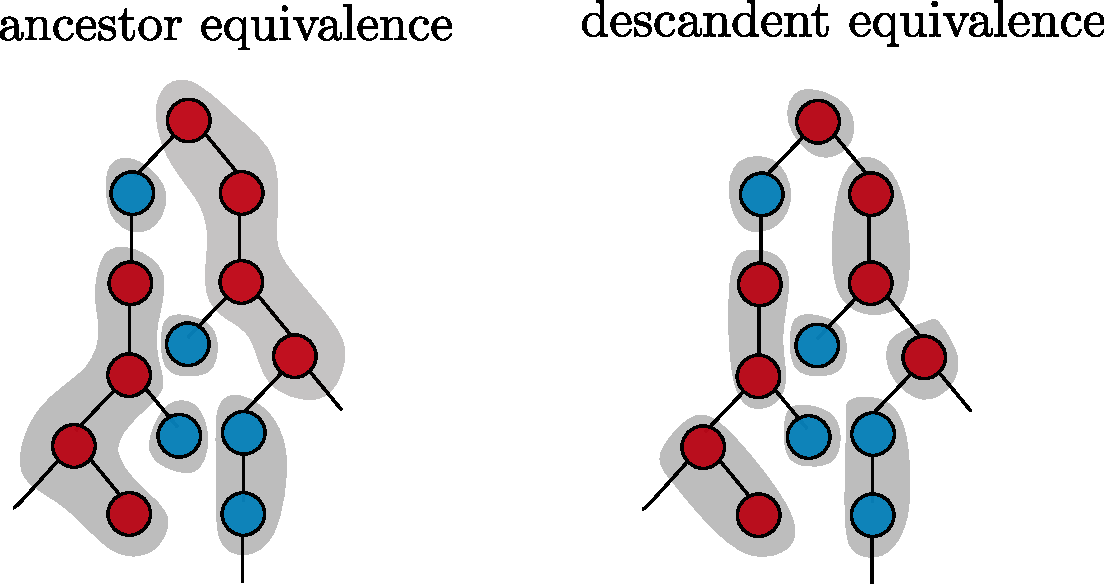
\includegraphics[scale=.3]{facto-up-down.pdf}
        \end{center}
        Both ancestor and descendant equivalences are factorisations; and in each case equivalence classes contain only nodes of same type.  The function $\ancfact$ maps a term to (the term of terms corresponding to) its ancestor equivalence relation, likewise we define $\decfact$ for  descendant factorisations.
    
        \subsubsection{Pre-order traversal.} The preorder traversal function  
        \begin{align*}
            \ranked{\preorder : \tmonad \Sigma \to \reduce 1 \tmonad (\rSigma + 0 + 2)}
        \end{align*}
        is the natural extension -- from trees to terms -- of the depth-first traversal, as explained below (the nullary grey nodes represent the labels from $\ranked 0$, and the binary grey nodes represent the labels from $\ranked 2$):
        \begin{center}
        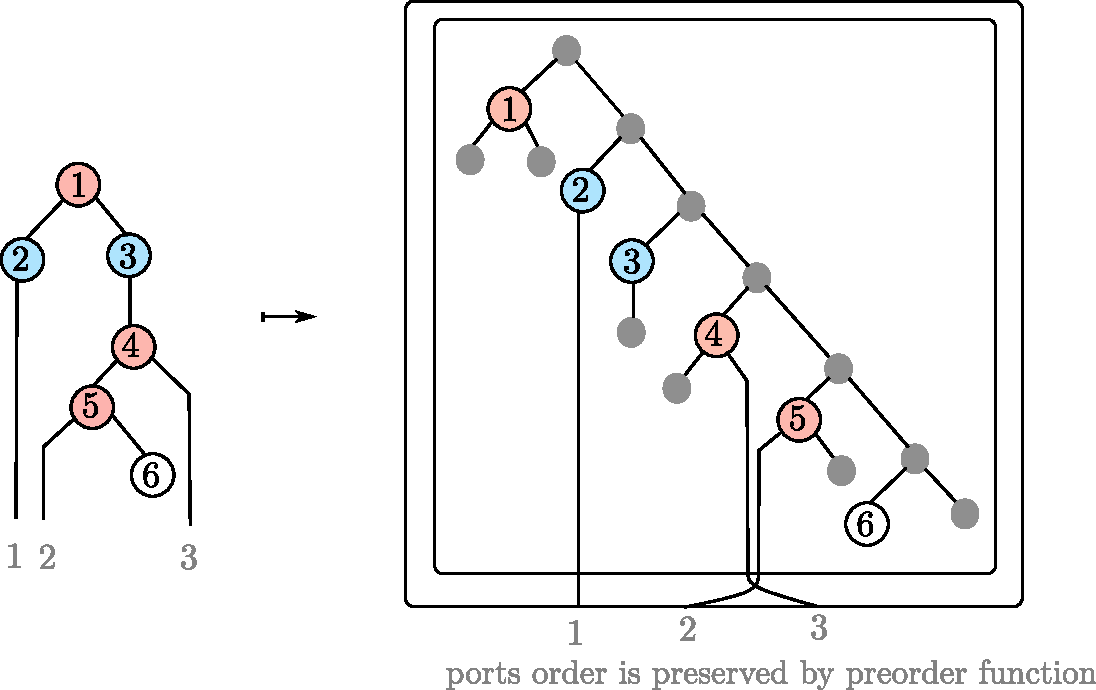
\includegraphics[scale=.34]{preorder.pdf}
        \end{center}
The $\preorder$ function respects the input port order, this is the reason  why we have a fold $\reduce 1$ in the output type. 

\subsubsection{Unfolding of the matrix power}
\label{sec:unfolding}
The final prime function is called monotone unfolding. The general idea is that this function unpacks a representation of several trees inside a single tree.  Before describing this function in more detail,  we introduce some notation.
\begin{definition}
    [Matrix power] For $k \in \set{1,2,\ldots}$ define the $k$-th matrix power\footnote{
        The name  matrix power is based the matrix power in  universal algebra (for the latter, see~\cite{Taylor1975} or~\cite{szendrei1990simple}). Roughly speaking, the restrictions that we place on the original definition correspond to the single-use and monotone conditions from Definition~\ref{def:stt}. 
     } of a ranked set $\rSigma$ 
to be 
\begin{align*}
 \mati k \rSigma \quad \eqdef \quad \ranked{\reduce k \rSigma^k}.
\end{align*}
\end{definition}
Here is a picture of elements in the third matrix power:
\mypic{102}
We use the name \emph{registers} for the coordinates $1,\ldots,k$ in the $k$-th matrix power. This terminology will be motivated later on in the paper, where the coordinates of the matrix power will correspond to registers in transducer. 


\begin{figure}[]
    \mypic{101}    
    \caption{Unfolding the matrix power}
    \label{fig:unfold}
\end{figure}

An element of the $k$-th matrix power  can be seen as having a group of $k$ incoming edges, and each of its ports  can be seen as a group of $k$ outgoing edges. The idea behind  unfolding  is that it matches the $k$ incoming edges in a node with the $k$ outgoing edges in the parent port; it also removes the unreachable nodes. This is illustrated in Figure~\ref{fig:unfold}. A formal definition of the  unfolding operation  is given in the appendix.

There are two variants of the unfolding operation:
\begin{align*}
    \underbrace{\ranked{\tmonad \mati k{\Sigma} \to \mati k{( \tmonad \Sigma)}}}_{\text{general unfolding}} \qquad 
    \underbrace{\ranked{\tmonad \mati k{\Sigma} \to \termset + \mati k{( \tmonad \Sigma)}}}_{\text{monotone unfolding}} 
    \end{align*}    
The general variant is the one that we have just described. The monotone variant -- which is the one that is included in the prime functions from Figure~\ref{fig:not-explained} -- is explained below.



% For an element of the matrix power
% \begin{align*}
% a =    \tensorpair{a_1,\ldots,a_k}/f \in \mati k \rSigma,
%     \end{align*}
% define its \emph{rewiring function} to be  the function
%     \begin{align*}
%     \coprod_{i \in \set{1,\ldots,k}} \text{ports of $a_i$} \quad \to \quad  \underbrace{\text{(ports of $a$)} \times \set{1,\ldots,k}}_{\text{sub-ports of $a$}}
%     \end{align*}
% which is obtained by first interpreting of $a_i$ as one of the ports in the tensor tuple $\tensorpair{a_1,\ldots,a_k}$, and then applying the grouping function $f$. Here is a picture:
% \begin{center}
%     (todo picture)
% \end{center}
% For a node $v$ of the term $t$ and $i \in \set{1,\ldots,k}$, define the $i$-th sub-node of $v$ to be the pair  $(v,i)$. We define a tree structure on sub-nodes as follows. Let   $(v,i)$ be a sub-node, and let $a_i \in \rSigma$ be the $i$-th component in the label of node $v$.  The arity of the sub-node $(v,i)$ is inherited from $a_i$, and its children are defined as follows. Take a port $x \in \set{1,\ldots,\text{arity of $a_i$}}$.  Apply the rewiring function to $(i,x)$, yielding a pair $(j,y)$. Take the $y$-th child of node $v$, call it $w$. The $x$-th child of $(v,i)$ is defined to be $j$-th sub-node of the $y$-th child of $v$.

% The unfolding of $t$ is  defined using the above tree structure. For $j \in \set{1,\ldots,k}$, the root of $t_i$ is the $i$-th sub-node of the root of $t$. The nodes in $t_i$ are all of the sub-nodes of $t$ that can be reached from this root by the child relation defined above, with the corresponding tree structure. Finally, 

\paragraph*{Monotone unfolding.} The general unfolding operation is too powerful to be included in the derivable functions. To see the problem, consider the following example, where two registers are swapped in each node of the input tree:
\mypic{108}
For inputs with an odd number of swaps (as in the above picture), the output of unfolding has a white leaf in the first register, and for inputs with an even number of swaps, the output has a white leaf in the first register. This shows how  general unfold can simulate  a certain amount of modulo counting, and therefore cannot be captured by first-order transductions. In fact, as we will see later in Theorem~\ref{thm:chain-transductions} -- having general unfold would lead to a more general class of transductions, corresponding to a fragment of \mso called \emph{chain logic}.

To avoid the problems with cyclic swaps, we impose a monotonicity restriction.  Let  $a \in \mati k \rSigma$ be an element of the matrix power,  let $p,q \in \set{1,\ldots,k}$ be registers, and let  $i$ be a port of $a$. We write $
     q \to_i p$
if register $q$ in the $i$-th outgoing edge  is connected to  register $p$ in root, as described in the following picture:
\mypic{109}
One can see that $\to_i$ is a partial function from $\set{1,\ldots,k}$ to $\set{1,\ldots,k}$. We call it the  \emph{twist function of the $i$-th port}. For example, the twist function in of the unique port in 
\mypic{110}
swaps registers $1$ and $2$. The idea behind monotone unfolding is to prohibit such swapping. Call  element of the matrix power  \emph{monotone} if for every port, its twist functions is monotone (when restricted to inputs where it is defined). The \emph{monotone unfolding} function is then defined as follows: if the input contains at least one label which is non-monotone, then the output is the error value $\termset$, otherwise the output is the same as for the general unfolding.

\paragraph*{Is unfolding derivable?} The  prime functions in our main theorem  are meant to be simple syntactic rewritings. It is debatable whether the  unfolding operation can be called a simple syntactic rewriting. For example, proving that monotone unfolding is a first-order transductions requires some non-trivial effort, including an invocation of the Sch\"utzenberger-McNaughton-Papert theorem about first-order logic on words being the same as counter-free automata~\cite[Theorem 10.5]{McNaughtonPapert71}. From this perspective, one can naturally ask: is it possible to break down monotone unfolding into simpler primitives?
In the appendix, we devote considerable resources to answering this question. We propose one new  datatype
\begin{align*}
\shallowterm \rSigma \rGamma \quad \eqdef   \quad \ranked{\coprod_{\black{a \in} \rSigma} } \overbrace{\ranked{\Gamma \otimes \cdots \otimes \Gamma},}^{\text{arity of $a$ times}}
\end{align*}
which represents trees of depth two, together with seventeen additional prime functions, which can be called syntactic rewriting without stretching the reader's patience. Then, we show that monotone unfolding can be derived, in the presence of  the new datatype and functions. The proof of this result is one of the main technical contributions of this paper, and takes half of the appendix.

% Suppose that the input is 
% \begin{align*}
% (\tensorpair{a_1,\ldots,a_k}/f)\tensorpair{t_1,\ldots,t_n} \in 
% \end{align*}
% First apply the unfold operation to the smaller trees $t_1,\ldots,t_n$, yielding trees
% \begin{align*}
% \tensorpair{t_{11},\ldots,t_{1k}}/f_1 \quad \cdots \quad  \tensorpair{t_{n1},\ldots,t_{nk}}/f_n
% \end{align*}
% For $i \in \set{1,\ldots,k}$ construct a term $s_i$ as follows. The root label is $a_i$. If the arity of $a_i$ is $n_i$, then let $t_{ij}$ be the tree 
% For two ranked sets $\rSigma$ and $\rGamma$, define 
% \begin{align*}
% \shallowterm \rSigma \rGamma \quad \eqdef   \quad \ranked{\coprod_{\black{a \in} \rSigma} } \overbrace{\ranked{\Gamma \otimes \cdots \otimes \Gamma}}^{\text{arity of $a$ times}}
% \end{align*}
% \begin{align*}
%     \ranked{
%         \xymatrix{
%             \shallowterm{\mati k \rSigma} {\mati k \rGamma}  \ar[r] & \mati k {(\shallowterm \Sigma \Gamma)}.
%         }
%     }
% \end{align*}
% \begin{align*}
% \tmonad \rSigma = \redset{ \portletter} + \shallowterm \rSigma {\tmonad \rSigma}
% \end{align*}


% to be the set of terms over alphabet $\rSigma + \rGamma$, where the 
% % , this operation of determining the dependency tree is what we call \emph{unfolding}. We illustrate it by the following example 
% % \begin{center}
% % 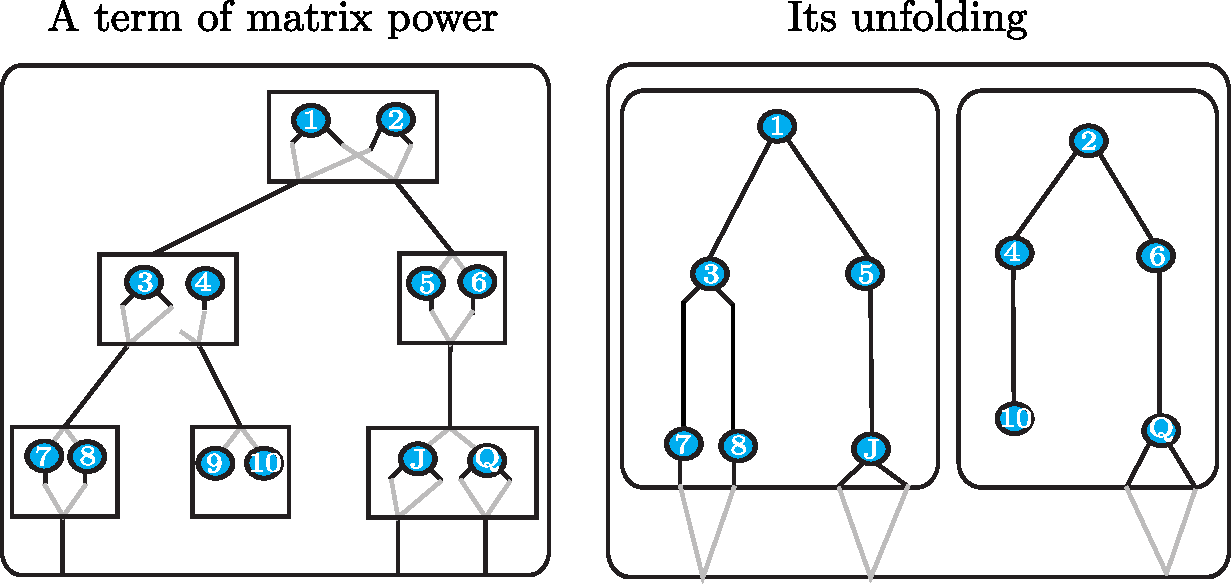
\includegraphics[scale=.38]{unfold-matrix-power}
% % \end{center}
% %  which is defined as follows by induction on the size of the input term. 
% If the input is an empty term, then the output is this term:
% \begin{center}
% \includegraphics[scale=.3, page=83]{pics.pdf}
% \end{center}
% % Otherwise, if the input is a nonempty term $(a_1,\ldots,a_k)/f)(t_1,\ldots,t_n)$. 
% Apply unfolding inductively, yielding 
% For $i \in \set{1,\ldots,k}$ define $s_i$ to be the tree where the root label is $a_i$, and the children are obtained ... 

% Consider an edge in the tree $t$, which connects either a node with one of its children, or a node with one of the ports. For $i \in \set{1,\ldots,k}$, define the $i$-th source of the edge to be the node ; likewise define the $i$-th target of the edge to be the $i$-th subnode of $s$.  For a node $x$ in $t$ and $i \in \set{1,\ldots,k}$, define the $i$-th subnode of $x$ to be the label (from $\rSigma$) in the $i$-th coordinate of the label of $x$.  For a subnode, define its \emph{outgoing edge} to be the edge of the tree 

% Define a \emph{inport} of $s$ to be a pair (node of $s$, number in $\set{1,\ldots,k$}). Define an \emph{outport} to be a pair (node $s$, number in $\set{1,\ldots,k}$, number in $\set{1,\ldots,\text{arity of $s$}$}). 

% \begin{align*}
% \underbrace{\text{(nodes in $s$)} \times \set{1,\ldots,k}}_{\text{sub-nodes}} 
% \qquad
% \underbrace{\text{(edges in $s$)} \times \set{1,\ldots,k}}_{\text{sub-edges}}
% \end{align*}
% For a sub-node $(v,i)$, define its label to be the label in $\rSigma$ of the $i$-th coordinate in the label of $v$. Define the arity of the sub-node to be the arity of its label. If a sub-node has arity $n$, and $j \in \set{1,\ldots,n}$, then the $j$-th out-going sub-edge of the sub-node is defined in the natural way. 


% Consider an  element
% \begin{align*}
% (a_1,\ldots,a_k)/f  
% \end{align*}

% \begin{align*}
% \coprod_{i \in \set{1,\ldots,k}} \set{1,\ldots,\text{arity of $a_i$}} \qquad \to \qquad \set{1,\ldots,n} \times \set{1,\ldots,k}
% \end{align*}
% For $i \in \set{1,\ldots,k}$ and a node node $v$ in the tree $s$ which has label $(a_1,\ldots,a_k)/f$. For $j \in \set{1,\ldots,\text{arity of $a_i$}}$. Let define the $j$-th child of to be the 

% Define a \emph{sub-edge} to be a pair (edge in $s$, number in $\set{1,\ldots,k}$). Define a \emph{sub-node} to be a pair (node in $s$, number in )

% then the output is obtained by first applying unfolding to to the smaller terms $t_1,\ldots,t_n$, and then applying the following derivable function, which we call \emph{shallow unfold}. 
% \begin{align*}
%     \ranked{
%         \xymatrix{
%             \shallowterm{\mati k \rSigma} {\mati k \rGamma}  \ar[r] & \mati k {(\shallowterm \Sigma \Gamma)}.
%         }
%     }
% \end{align*}
% Here is a picture of unfolding for shallow terms:
% \begin{center}
% 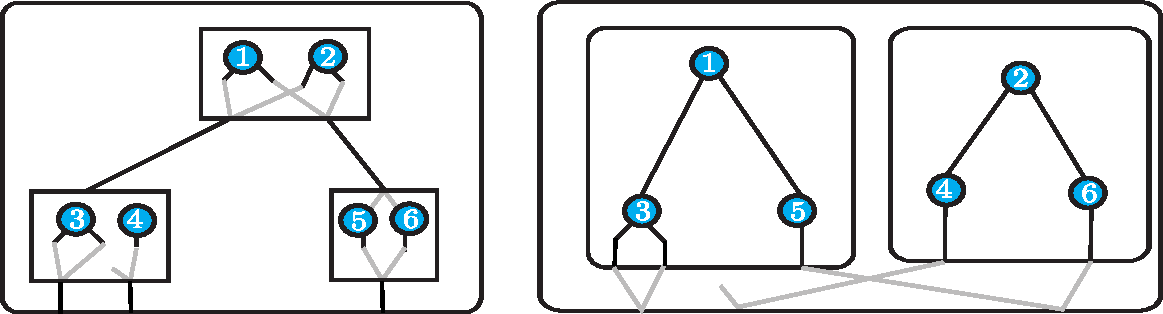
\includegraphics[scale=.4]{unfold-shallow}
% \end{center}
%\subsubsection{Unfolding}
%The general idea behind the  unfolding operation 
%\begin{align*}
%\ranked{
%    \unfoldsmall : \shallowterm {(\reduce k   \Sigma)} {\Gamma^k} \to \reduce 1 (\shallowterm \Sigma \Gamma)
%}
%\end{align*} 
%is to eliminate a $k$-fold by matching it with a $k$-th power. 
%The unfolding operation is explained in the following picture for $k=2$: 
%        \begin{center}
%        \includegraphics[scale=.36]{shallow-unfold.pdf}
%        \end{center}


% One of the main results in this paper will be  that an iterated version of the unfold operation, of type
% \begin{align*}
% \ranked{    \tmonad (\reduce k \Sigma^k) \to \reduce k (\tmonad \Sigma)^k,}
% \end{align*}
% can be derived from the other operations. 

% The formal definition is 
% \begin{align*}
% (a/f) \tensorpair{\tensorpair{b_{1,1},\ldots,b_{1,k}},\ldots,\tensorpair{b_{n,1},\ldots,b_{n,k}}} \qquad \mapsto \qquad 
% (a\tensorpair{b_{f(1)},\ldots,b_{f(\arity a)}})/g
% \end{align*}
% where $g$ is defined so that it matches ...

\noindent\begin{example}\label{ex:filter} 
 To get a feeling for the prime functions and combinators, we derive the function
$$ \ranked{f:\tmonad (\rSigma+\rGamma)\to\tmonad \rSigma}$$
discussed earlier, which erases the elements of $\rGamma$ from the input term, where $\rGamma$ is a finite set of unary symbols. 

Consider the prime function $\ranked{\unit:\rSigma\to\tmonad\rSigma}$ and the constant function $\ranked{\epsilon:\rGamma\to\tmonad\rSigma}$ which associates to every element of $\rGamma$ the empty term. The function $\ranked{\epsilon}$ is prime because its domain is finite. We start by lifting $\ranked{\unit}$ and $\ranked{\epsilon}$ to the type constructor $+$, then we compose the result with the prime projection function as follows
\begin{align*}
\xymatrix{
    \ranked{\rSigma+\rGamma}\quad \ar[r]^-{\ranked{\unit+\epsilon}} & \quad \ranked{\tmonad\rSigma+\tmonad\rSigma}\ar[r]^-{} &\tmonad\rSigma
},
\end{align*}
We lift the obtained function to terms, and compose it with the $\flatt$ function to obtain our function $\ranked{f}$.  
\end{example}

More examples of derived functions are given in Appendix.~\ref{sec:AppendixExamples}.

